\documentclass[12pt]{article}
%\usepackage[showframe]{geometry}% http://ctan.org/pkg/geometry
\usepackage{lipsum}% http://ctan.org/pkg/lipsum
\usepackage{multicol}% http://ctan.org/pkg/multicols
\usepackage{graphicx}% http://ctan.org/pkg/graphicx
\usepackage{float}
\usepackage{fancyhdr}
\usepackage{titling}
\usepackage{subcaption}
\usepackage{indentfirst}
\usepackage{booktabs}
\usepackage{multirow} 
\usepackage{setspace} \doublespacing
\usepackage{mathptmx}
\usepackage{amsmath}
\usepackage[backend=biber, style=apa,]{biblatex}
\usepackage{hyperref}
\usepackage{indentfirst}
\usepackage{float}

\pagestyle{fancy}
\doublespacing

%\addbibresource{/mnt/c/Users/woute/projects/Thesis_endstop/MyLibrary.bib}
% \addbibresource{/home/wouter/projects/Thesis_endstop/latex_endstop/MyLibrary.bib}
\addbibresource{MyLibrary.bib}

\hyphenpenalty=1000
\tolerance=2000

\fancyhead{}
\fancyfoot{}
\fancyfoot[R]{\thepage}
\renewcommand{\headrulewidth}{0pt}

\setlength{\droptitle}{-10em}   % This is your set screw

\begin{document}

\begin{titlepage}
\centering

% Adjust font size and family as needed
{\LARGE\bfseries Local Circuit Structure of Mouse Visual Cortex for Generating Illusory Contour Responses\par}

\vspace{5pt} % Adjust space between title and figure as needed

% Include the figure

\includegraphics[width=0.5\textwidth]{figures/donders_logo.png}

\includegraphics[width=0.5\textwidth]{figures/uva_logo.png}


\vspace{20pt} % Adjust space between figure and author/date as needed

% Author and Date
{\Large Wouter Kroot\par}
\vspace{5pt} % Adjust as needed
{\Large April 2024\par}
\vspace{5pt}
{\Large Supervisor: Prof. dr. P.H.E. Tiesinga}

\end{titlepage}

% Rest of the document starts here
\newpage

% Abstract
\begin{abstract}
  \lipsum[1]
\end{abstract}

\newpage

\section{Introduction}
\subsection{Illusory contour and visual segmentation.}
The representation and identification of visual contours is an essential step in order to perceive coherent objects with respect to each other and the background.
In some cases, visual contours are clearly defined, e.g., by a luminance contrast that indicates a discontinuity. In other cases, other figures occlude contours, 
and objects must be partly inferred from locally available visual cues. Interestingly, particular stimulus configurations can give rise to the perception of contours 
that are not physically present. For example, the 'abutting grating' and 'Kanizsa' illusions (Figures 1 and 2). These illusory contours are a product of visual interpolation that signals the presence of an occluding figure. Although the perception of these geometrical shapes is seemingly simple, both illusions require a process that analyses the discontinuities of the inducing lines and assesses their relation towards each other. Typically, an illusory line is only formed when the connected edges form a closed contour and are interpreted as part of the foreground. Since these illusory contours are not physically present and are a direct product of our neural circuitry, illusory contours can  effectively be used to investigate the underlying neurophysiological interactions necessary to make perceptual inferences. Although there are many different stimulus configurations  that can elicit illusory contours, neurophysiological research has mainly focused on the abutting grating illusion and the Kanizsa triangle illusion. The results of both illusions will be discussed since their underlying neural mechanisms are likely similar. In order to make the results from current simulations as clear as possible, the choice was made only to use the abutting grating illusion and not Kanizsa. Furthermore, the goal of the current model is to further explain the cortical representation of illusory contour by explicitly modelling receptive fields along the visual pathway, trying to account for the most important constraints posed by mammalian neurophysiology.

\bigbreak

\noindent The initial neuronal evidence of illusory contours was identified in V2 neurons of alert rhesus macaques \autocite{vonderheydtMechanismsContourPerception1989}.
%\autocite{vonderheydtMechanismsContourPerception1989}. %(von der Heydt \& Peterhans, 1989). 
To elicit the abutting gratings illusion, offset lines were presented in an abutting pattern with overlapping ends (see Figure 1). This research highlighted 
a distinct difference between the primary visual  cortex (V1) and the secondary visual cortex (V2). It was discovered that V1 plays a minimal role in the representation of illusory contours, with nearly all orientation-selective neurons (59 out of 60) showing no activity related to the orientation of the illusory contours. In contrast, a significant number of neurons in V2 (45 out of 103, or approximately 44\%) did respond to the orientation of illusory contours, signifying that V2 represents the initial cortical area where illusory contours are detected. Furthermore, it was observed that many V2 neurons displayed similar orientation tuning for both real and illusory contours. However, there were also neurons that responded to both real and illusory contours at  orientations diverging by up to 90 degrees. These observations demonstrate the visual system's capacity to represent information beyond the mere activation by direct sensory input. Illusory contours entail advanced processing, wherein the brain infers the existence of contours from the local visual cues provided and sends feedback to the lower visual areas. 
This inferential process is essential for forming a coherent perception of the visual environment, allowing the visual system to interpolate missing segments and interpret ambiguous or incomplete visual scenes.
  
\begin{figure}
    \centering
    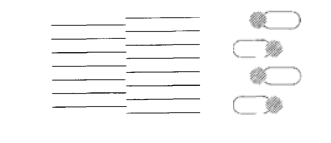
\includegraphics[width=0.95\textwidth]{figures/simple_abutting.png}
    \caption{Abutting grating illusion (Soreano et al., 1996), the offset between the lines gives the impression of a vertical contour overlapping the horizontal inducers. 
    The proposed neural mechanism is the integration of endstopped cells, which can be characterised by an elongated excitatory receptive field and inhibitory endzones.}
    \label{fig:figure_1}
\end{figure}

\bigbreak
\subsection{Neural mechanism macaque V4 and mice V1-LM.}
Macaque V2 cells' showed that their tuning to illusory contours is not necessarily the same as the orientation tuning to real contours, which suggests a potential mechanism where feedback signals may determine V2 cells' orientation selectivity towards illusory contours. If the orientation tuning to illusory contours were indeed a result of feedback, a direct implication would be that higher visual areas might be unable to distinguish between real and illusory contours. This hypothesis has been examined, with area V4 in the macaque identified as a crucial integration point where both real and illusory contours are represented equivalently \autocite{panEquivalentRepresentationReal2012}. Through the use of optical imaging and single-cell recordings to compare neural activity elicited by real and illusory contours across areas V1, V2, and V4, it was found that activities in V1 and V2 predominantly relate to the encoding of local spatial features of the inducers, rather than the global orientation of the illusory contour. Meanwhile, V4 processed both real and illusory contours similarly, indicating that hierarchical interactions might govern the global orientation processing of illusory contours. This suggests that feedback mechanisms could account for the selective stimulation and orientation tuning of V2 cells in response to illusory contours.
\bigbreak

\noindent Additional support for the vital role of feedback in the representation of illusory contours is provided by studies illustrating the interactions between V1 and the lateromedial visual area (LM) in mice during the perception of illusory contours \autocite{pakTopDownFeedbackControls2020}. These studies trained mice to differentiate between stimuli with and without illusory contours, linking their behaviour to neural activity (Figure 2). Given the extensive genetic tools available for mice that allow for the precise recording and stimulation of specific cells, they are exceptionally well-suited for investigating the hierarchical processing that underpins perceptual inferences. The findings revealed that, akin to macaques, mice also exhibited a delay (30 ms) in the representation of illusory contours compared to those defined by contrast, suggesting that the processing of illusory contours involves a more complex integration of visual information than that of contours directly derivable from sensory input. Moreover, the representation of illusory contours in V1 was eliminated upon the silencing of LM through optogenetics, indicating a possible similarity in the processing relationship between V1 and LM in mice and that between V2 and V4 in macaques, which aligns with theories of recurrent processing \autocite{wyatteEarlyRecurrentFeedback2014}. Additionally, recent research \cite{shinRecurrentPatternCompletion2023} found that a specific subset of V1 cells in mice could complete the perception of an illusory contour when sufficiently stimulated. Employing decoding techniques and 2-photon stimulation, it was demonstrated that activating a particular set of V1 cells could suffice to generate the perception of illusory contours across the V1 network, even without any visual stimulus. These findings underscore the significance of recurrent activity in the representation of illusory contours and highlight the necessity for further investigation into how these cells are precisely targeted based on the configuration of inducing stimuli.

\begin{figure}[H]
    \centering
    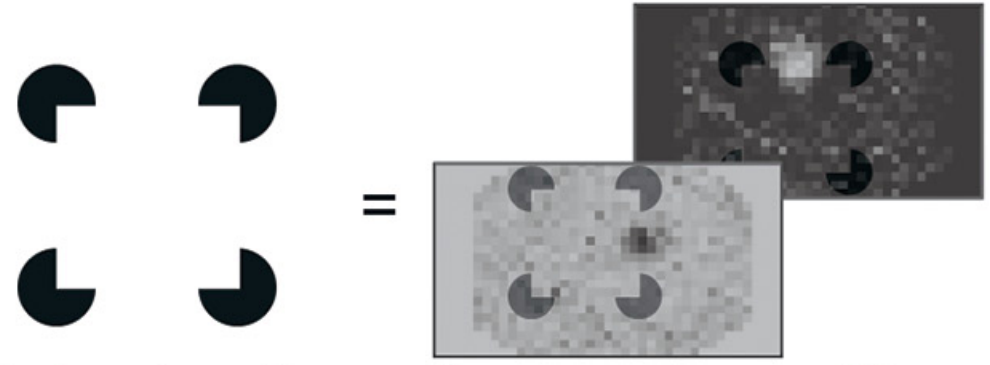
\includegraphics[width=0.95\textwidth]{figures/Kanizsa_Mice.png}
    \caption{Kanizsa illusion (Pak et al., 2020), four spatially synchronous pac-men that induce the impression of a white square overlapping four circles, inducing the percept of a not physically present contour. When presented to mice, orientation-selective cells show activity along the length of the illusory line.}
    \label{fig:simple_abutting}
\end{figure}

\bigbreak
\subsection{Endstopped cells fundamental to illusory contour representation.}
The abutting grating and Kanizsa illusions are both characterized by congruent illusory inducing points, identifiable by the presence of aligned line endings. Kanizsa inducers are considered more complex than abutting line inducers because each inducer point forms part of a corner, essentially two line ends meeting at an angle. In contrast, the abutting grating illusion is simpler, with its inducer points as single-line ends and, therefore, could be represented by a single endstopped cell \hyperref[fig:figure_1]{(figure 1)}.
Nonetheless, cells sensitive to length might be fundamental to encoding both illusions, known as endstopped cells. Initially classified by Hubel and Wiesel in the cat's primary visual cortex (V1) in 1969, these cells are orientation-tuned and exhibit inhibition when a line segment exceeds their excitatory receptive field, leading to their initial characterization as hypercomplex cells for their complex cell properties, such as stimulus polarity invariance, combined with inhibitory end zones \autocite{hubelRECEPTIVEFIELDSFUNCTIONAL1965}. Subsequent research revealed that a significant portion of V1 neurons exhibit endstopping to varying degrees  \autocite{deangelisLengthWidthTuning1994,jonesSurroundSuppressionPrimate2001,sceniakVisualSpatialCharacterization2001} across different species, including primates, cats, and mice. Computational models have shown that endstopping can sufficiently delineate figures from the background and reconstruct illusory contours \autocite{vonderheydtMechanismsContourPerception1989}, suggesting that endstopped cell integration might serve as a universal neural mechanism for segmenting the visual field and to generating illusory contours.

\textbf{Image segmentation between mice and macaque have different straties, luongo 2023, both are suitable for endstopping.}

\begin{figure}
  \centering
  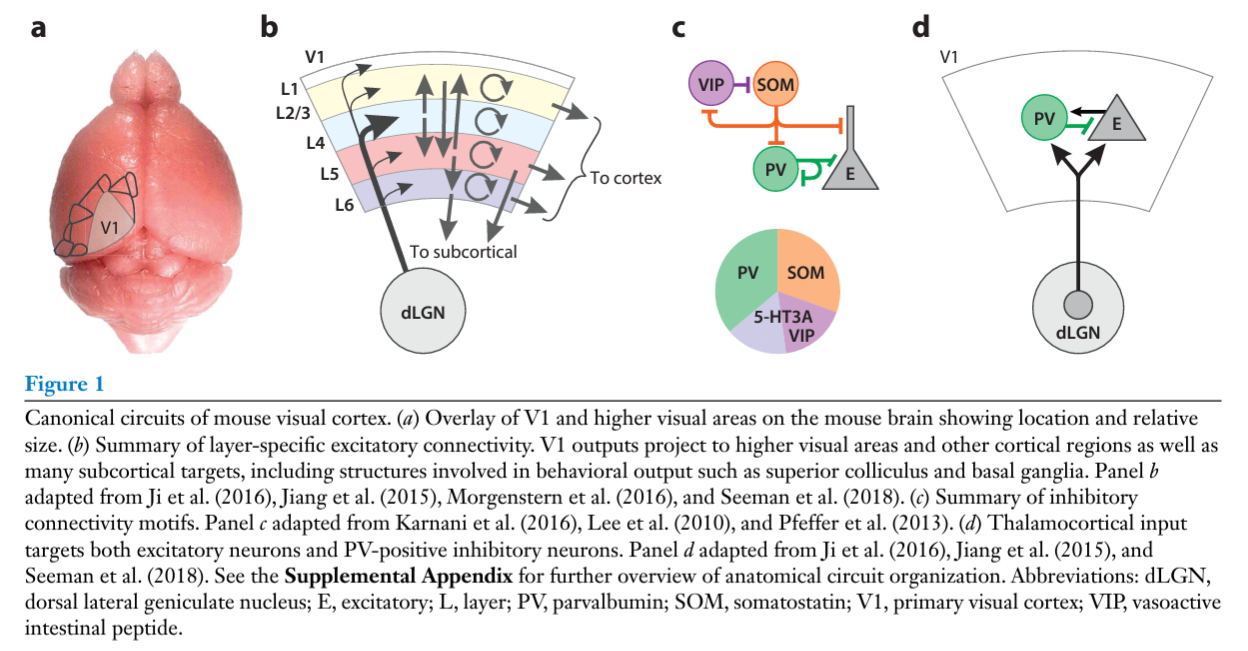
\includegraphics[width=1.0 \textwidth]{figures/Canonical_laminar_projection.png}
  \caption{laminar projections similar from apes and mice?, from Niell, Scanziaini, 2021 Annual Review}
  \label{fig:figure 3}
\end{figure}

\bigbreak
\subsection{Current study.}
Despite these insights, neurophysiological studies have largely overlooked how endstopping is integrated into higher visual areas for illusory contour perception. Previous computational simulations, while informative, have relied on feed-forward convolutions without accounting for biological constraints, such as direct inhibition to simulate negative end zones (Sillito \& Versiani, 1977), and have not incorporated feedback mechanisms now recognised as crucial for the representation of illusory contours in lower visual areas.

\noindent Addressing this gap, our current research endeavours to simulate endstopping using Leaky Integrate and Fire (LIF) neurons and to integrate endstopped microcircuits through population rate models to accurately represent the abutting grating illusion. Our findings shed light on the minimal microcircuit necessary to exhibit end-stop characteristics, further illuminating how the representation of illusory contours through recurrent activity is modulated by the orientation selectivity of endstopped cells in higher visual areas. By incorporating endstopped cells into a hierarchical model, we aim to elucidate the neural mechanisms underlying illusory contour perception and to provide a comprehensive understanding of how the visual system processes illusory contours.

\noindent This study investigates whether endstopping in V1 can occur solely through feedforward signals without direct inhibition or if a feedback mechanism is essential for activating inhibitory end zones. By simulating the representation of the abutting grating illusion via endstopped cell-driven recurrent activity, we explore the physiological constraints on integrating orientation-tuned endstopped cells in higher visual areas. Our goal is to elucidate how endstopped cells contribute to the perception of illusory contours and their integration within the visual cortex hierarchy. We hypothesize that endstopped cells are crucial for the representation of illusory contours and that their orientation tuning is modulated by feedback signals from higher visual areas. Our results will provide insights into the neural mechanisms underlying illusory contour perception and the hierarchical processing of visual information in the mammalian visual system.

\newpage
\section{Methods}
% Introduction that states that we used two models with a rationalisation of why
\noindent \textbf{Spiking neuron and population Model design.} \newline
To investigate the local circuit necessary for endstopping and how endstopping features can be used to generate illusory contours within the visual cortex of the mouse, the current study used two distinct computational frameworks. In the initial phase of the investigation, we utilised leaky integrate-and-fire (LIF) models to simulate the spatial and temporal integration of synaptic input, on the single-cell level. This approach provided a foundational understanding of the mechanisms underpinning orientation selectivity, complex cell features such as polarity invariance, and endstopping. However, the current connectivity between LIF cells was set by hand, and the complexity and computational demands associated with the tuning of each neuron constrained the current study to shift towards population models for the subsequent phase of generating illusory contours. Nevertheless, the LIF network allowed an estimate of the necessary amount of cells needed to create a stable neural mechanism for endstopping, and the population models could abstract this behaviour into a computationally tractable form, enabling the simulation of illusory contour generation efficiently. 

\bigbreak
\subsection{Simulating the Local Circuit for Endstopping using the BMTK.}

To stimulate endstopping behaviour the Brain Modeling Toolkit was utilised to define and connect nodes. To construct an architecture of spiking point neurons it is necessary to initilialise an instance of the NetworkBuilder class provided by the BMTK. The current example will create a network for the dLGN and a network for V1. To present the visual stimuli and connect nodes from the LGN to V1, the Brain Modelling Toolkit was used. This simulation pipeline processed visual information through a series of steps with increasing complexity, starting with presenting the visual stimulus. Visual stimuli were dynamically presented through a three-dimensional array format (t, y, x). Each entry along the first dimension time (t) is a frame with input organised along the vertical (y) and horizontal (x) dimensions. By following these steps, you can effectively use the Brain Modeling Toolkit to create complex neural networks. The toolkit's flexibility allows for precise control over the spatial arrangement and connectivity of neurons, facilitating the modeling of intricate neural circuits and their dynamic behaviors. This guide demonstrates the process of defining, connecting, visualizing, and saving neural networks using BMTK, providing a robust framework for neural network modeling and simulation. An important aspect of BMTK is its support for different simulation environments. In this context, we used two distinct types of simulations: filternet and pointnet. Filternet is employed to simulate the LGN, focusing on the filtering properties of LGN neurons and their responses to visual stimuli. This separate simulation environment is particularly suited for capturing the dynamics of large-scale LGN networks and their pre-processing role in the visual pathway. The importance of using filternet lies in its ability to model the initial stages of visual processing, where the LGN acts as a relay station, refining and filtering visual information before it reaches the cortex. This simulation environment allows for detailed analysis of how LGN neurons process various visual inputs and contribute to the overall visual perception.
\bigbreak
\noindent On the other hand, pointnet is used to simulate the V1 network with the NEST simulator. NEST is well-suited for modeling spiking neural networks and supports the integration of point-neuron models, making it ideal for simulating the detailed spiking activity and synaptic interactions within the V1 network. By using pointnet, we can leverage NEST's capabilities to simulate the complex dynamics of V1 neurons, including their interactions and the resultant network behavior. The importance of using pointnet lies in its ability to model the cortical processing of visual information, where the integration of inputs from the LGN and the intrinsic cortical circuitry results in the emergence of complex visual features such as orientation selectivity and phase invariance. By separating the simulations into filternet for the LGN and pointnet for the V1 cortex, we can more accurately model the distinct roles these regions play in visual processing. Filternet allows for a focused examination of the LGN's filtering mechanisms, while pointnet provides a detailed simulation of cortical processing dynamics. This approach ensures that each component of the visual pathway is modeled with the appropriate level of detail, leading to more accurate and comprehensive simulations of visual processing.

% Overview figure
\begin{figure}[H]
  \centering
  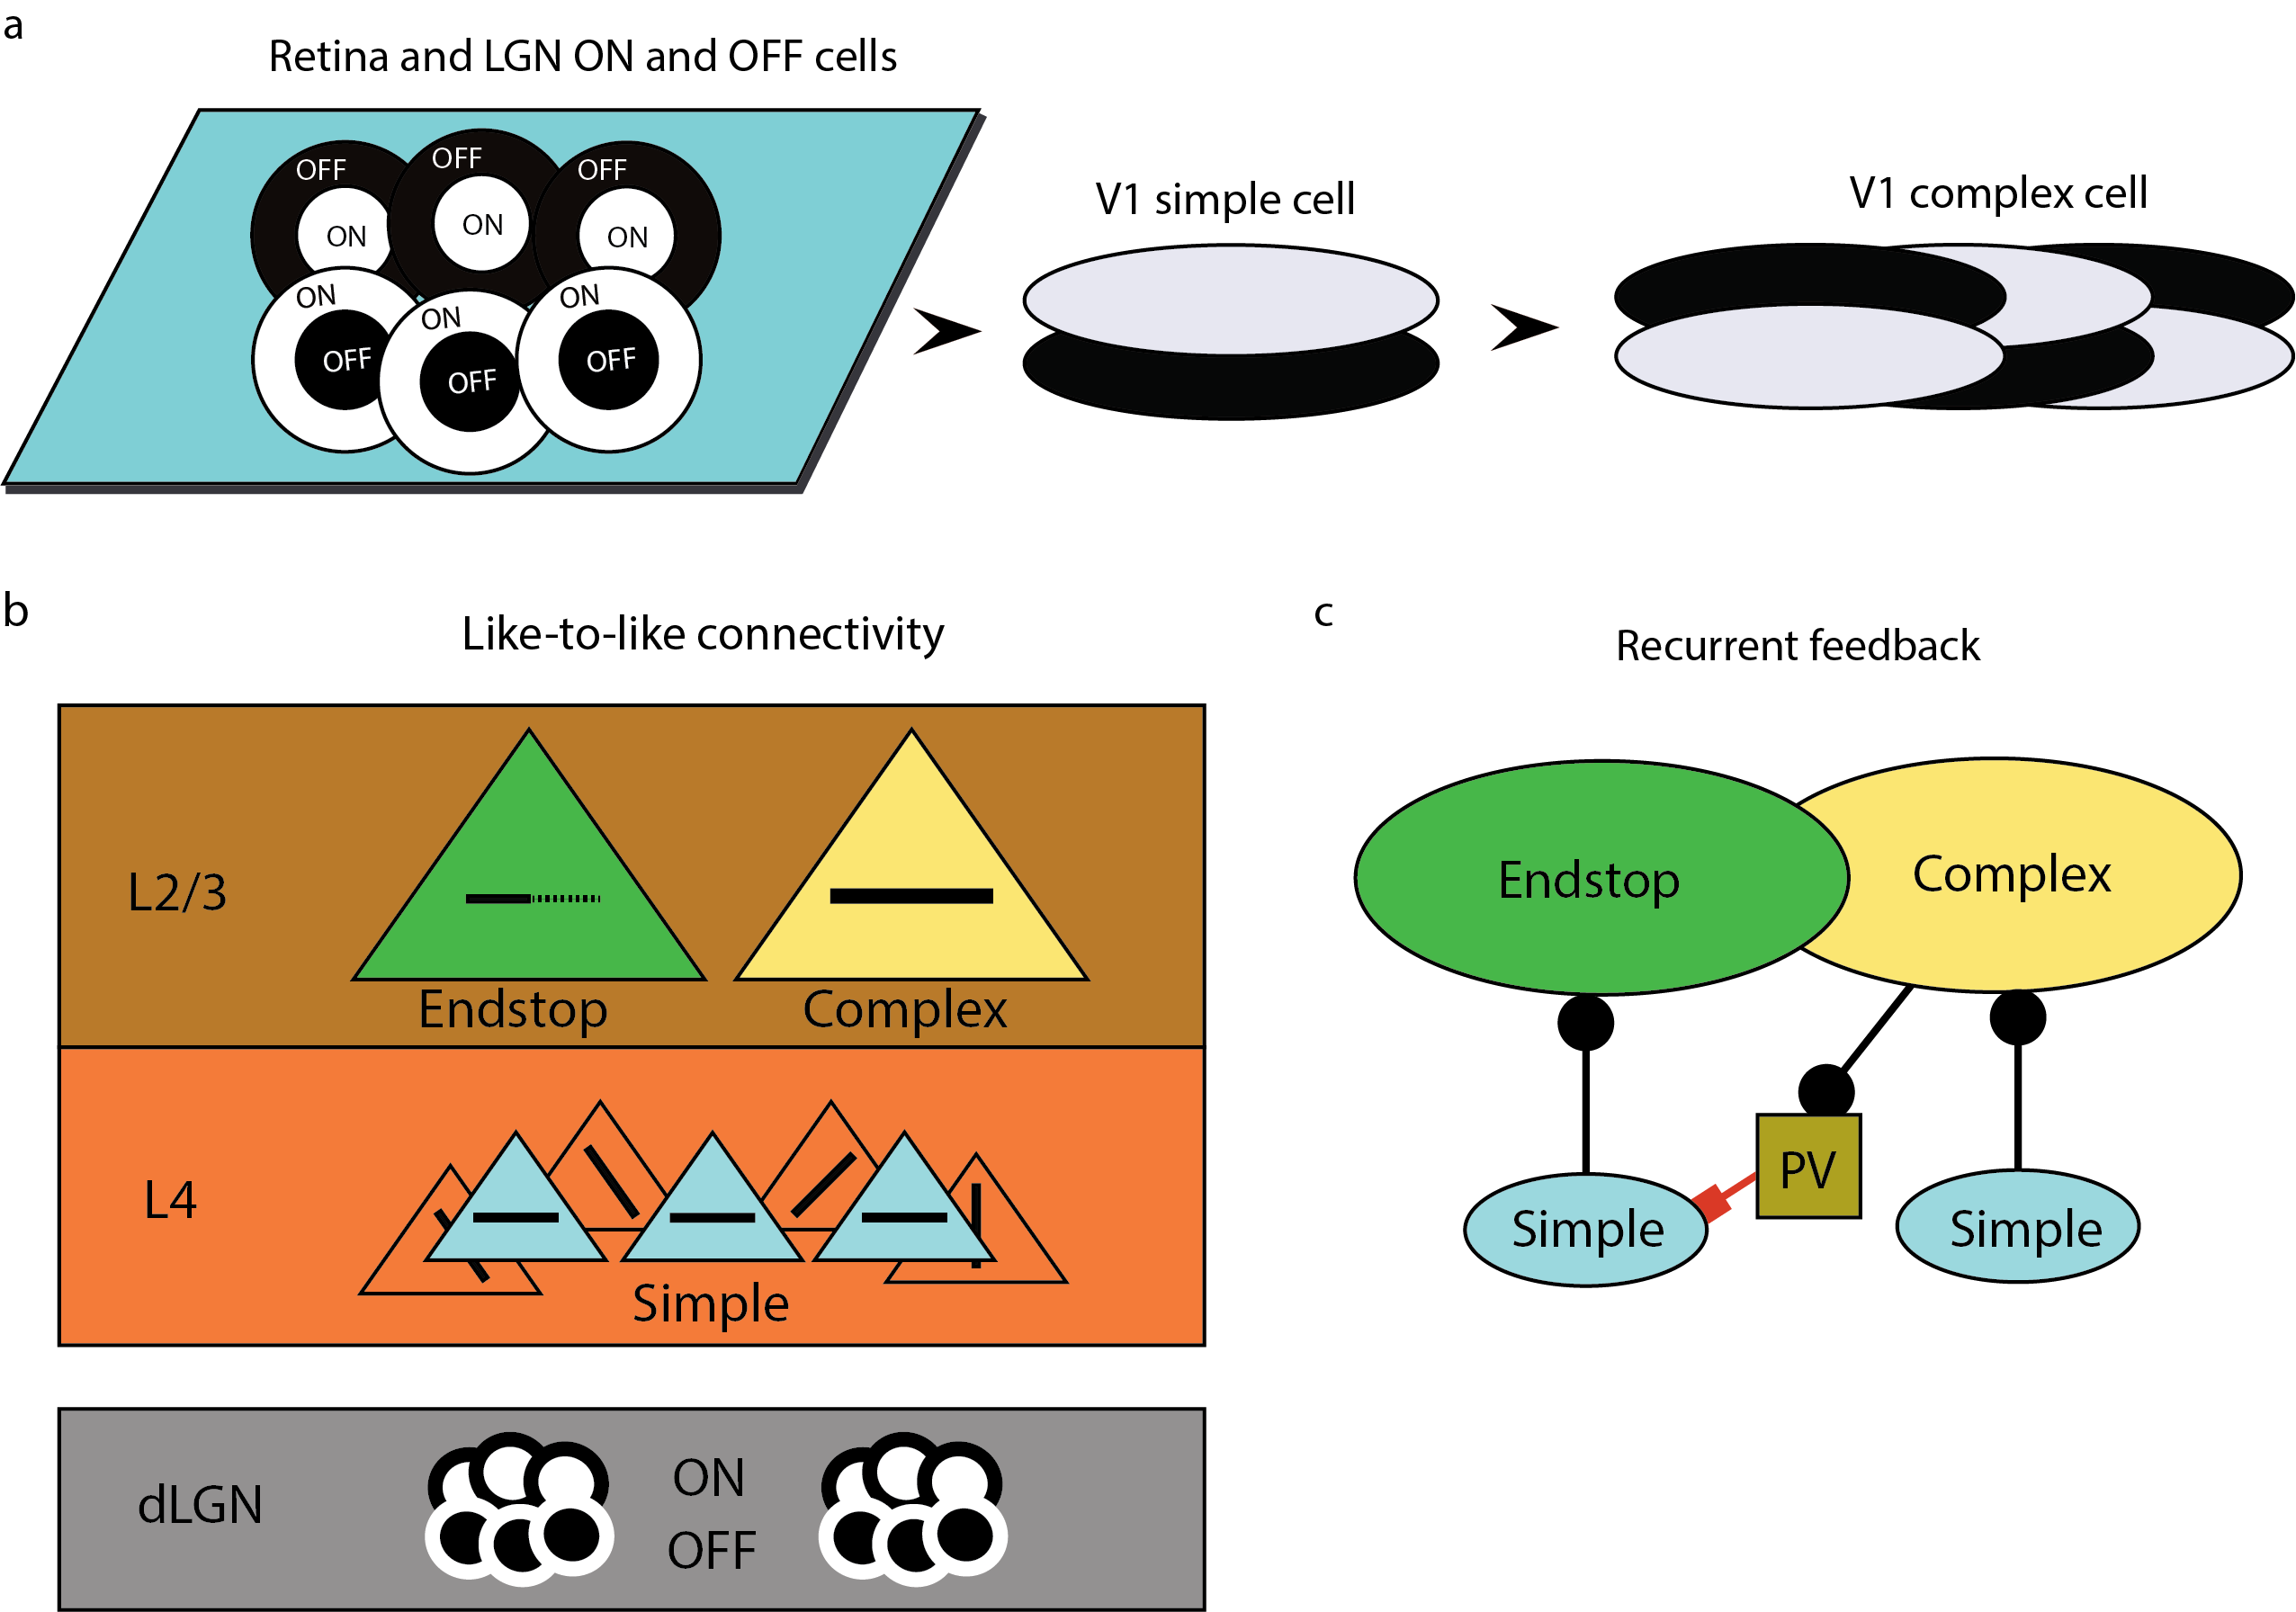
\includegraphics[width=1.0 \textwidth]{figures/Overview_Receptive_Field_Methods.png}
  \caption{Description}
  \label{fig:LIF_Overview}
\end{figure}


\subsection{dLGN during stimulus presentation}
The first relay station in the visual pathway is the dorsal Lateral Geniculate Nucleus (dLGN), which receives input from the retina and transmits visual information to the primary visual cortex (V1) for further processing. The dLGN processes visual stimuli through two distinct pathways: the ON and OFF pathways, which respond to increases and decreases in light intensity, respectively. These pathways are essential for encoding contrast and edge information in visual scenes, providing the initial processing steps that shape the neural representation of visual stimuli. To simulate the dLGN's response to visual stimuli, we used the Brain Modeling Toolkit (BMTK) to construct a network of dLGN cells and present monochromatic greyscale images to the network. The BMTK provides a flexible framework for building and simulating neural networks, allowing us to define the spatial arrangement of dLGN cells, their receptive fields, and their connectivity patterns. By presenting visual stimuli to the dLGN network, we can effectively simulate the translation of light input into neural signals, creating the first layer for contrast detection in the visual system.

Since we are interested in contrast, which is encoded in V1 rather than color, only monochromatic greyscale stimuli were shown. To transform this input array into neural signals, the dLGN was simulated as a linear-non-linear Poisson cascade model. First, visual input within the space of the receptive field of the LGN cell is convolved with a linear filter. Then a nonlinear function is applied to the output of the previous linear filter, giving the neuron's instantaneous spike rate as its output. Finally, this firing rate generates spikes according to an inhomogeneous Poisson process \autocite{moskovitzComparisonDeepLearning2018}.

The current dLGN model consists of two unit types, ON and OFF surround cells, optimized to closely mimic mammalian thalamic cells. The ON and OFF cells of the LGN converge on a layer of simple cells, effectively simulating layer 4 (L4) of V1 (Figure \ref{fig:LIF_connectivity}a). This dual pathway of ON/OFF cells is essential for the initial segregation of visual information, setting the stage for more complex edge detection and contrast processing within higher cortical areas.

We analyzed spiking features in response to static images. Therefore, we focused on modeling ON and OFF cells to have a predominantly sustained responses (sON and sOFF). We used the model templates in our node configuration to implement these cells in our network. The parameters for these cells were set based on values derived from electrophysiological recordings from the mouse dLGN, as reported by \autocite{durandComparisonVisualResponse2016} and \autocite{billehSystematicIntegrationStructural2020}.

\begin{figure}
  \centering
  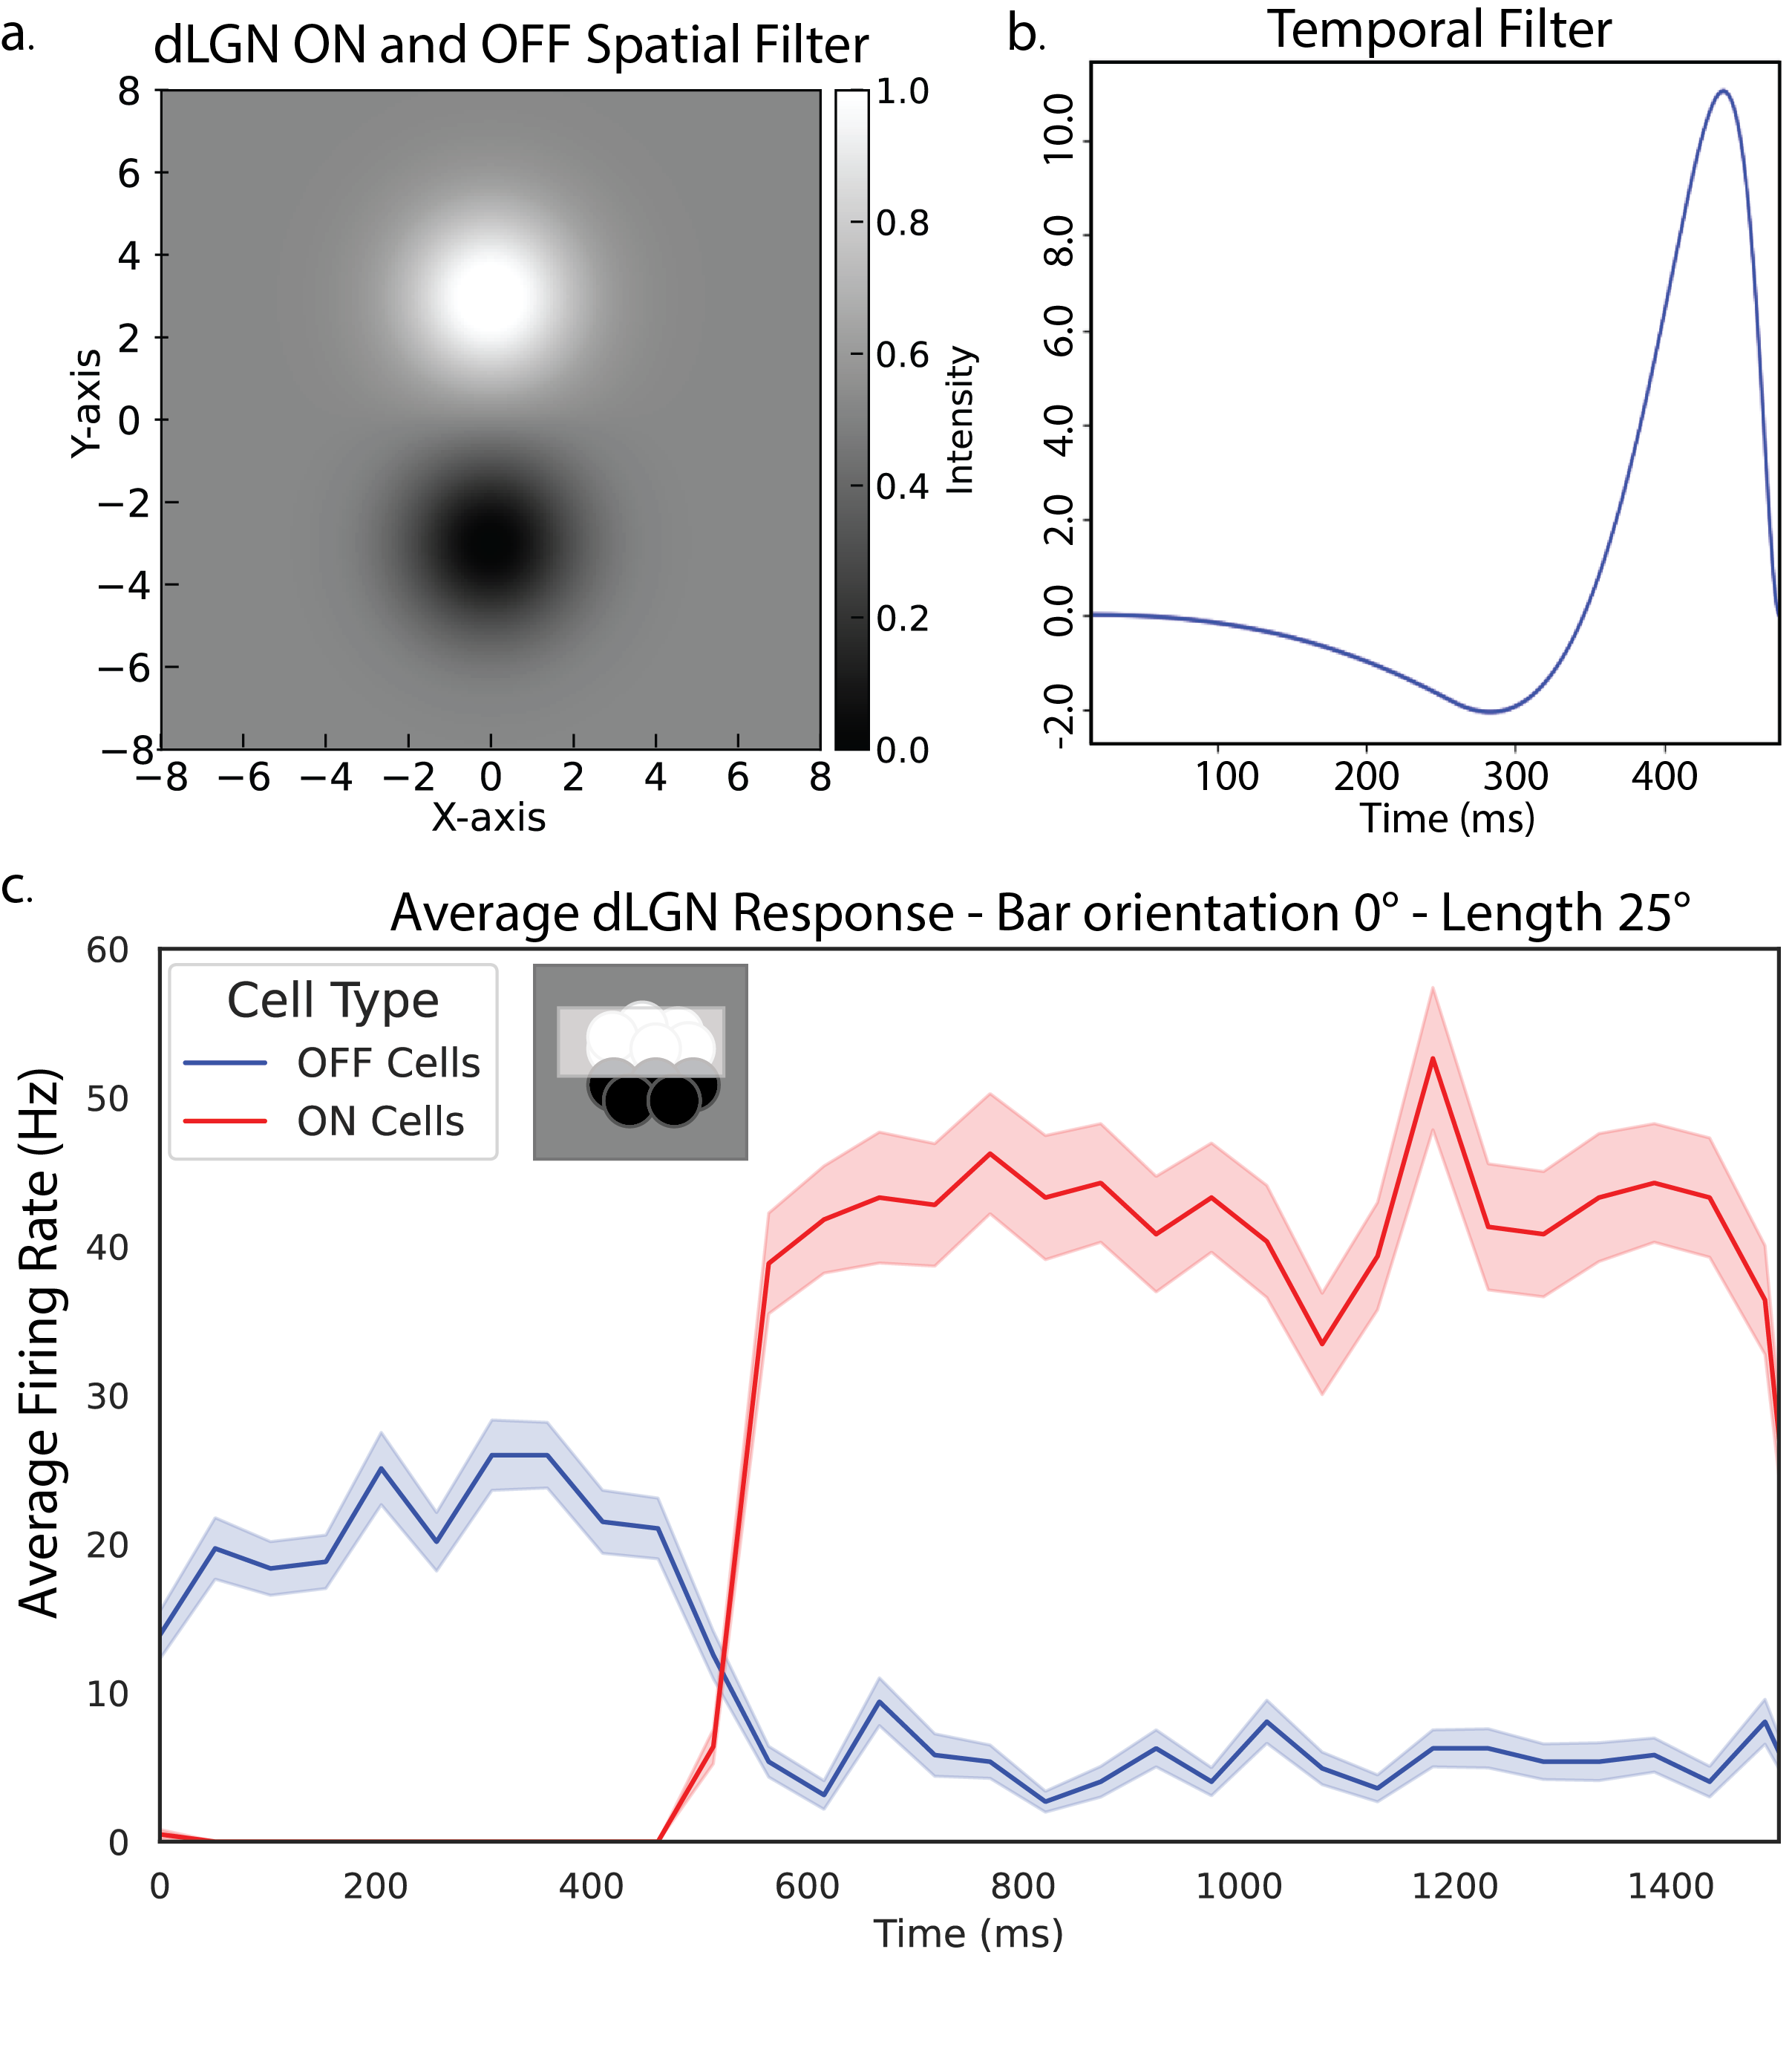
\includegraphics[width=1.0 \textwidth]{figures/lgn_response_fig.png}
  \caption{Description of the LGN cells response to monochromatic greyscale stimuli, light and black.}
  \label{fig:LIF_connectivity}
\end{figure}

\textbf{LGN and V1 parameters} For the spatial filtering of the receptive fields, we employed a Gaussian filter characterized by its spatial size and rotation. The default spatial size was set to 5.0 spatial degrees for both rows and columns, with a rotation of 0.0 degrees. The temporal filtering was managed using a double cosine filter. The parameters for this filter included weights, kpeaks, and delays. The weights parameter controlled the amplitude of the two peaks in the cosine filter, with the first value being greater than the second (weights[0] > weights[1]). The kpeaks parameter determined the spread of the peaks, ensuring the second peak had a greater spread than the first.

The delays parameter controlled the timing of the peaks, with delays[0] setting the delay for the first, larger peak and delays[1] setting the delay for the second, smaller peak. A smaller value for delays[0] resulted in a quicker initial response to brightness changes, while a larger value meant a slower initial response. Similarly, delays[1] determined how quickly the secondary response occurred, with smaller values indicating quicker secondary responses and larger values indicating slower ones. By carefully setting these parameters, we ensured that the LGN cells accurately modeled the sustained neural responses to both ON and OFF input necessary for our study.

\begin{table}[H]
  \centering
  \caption{Parameters and Weights for LGN and V1 Cells}
  \begin{tabular}{lll}
  \toprule
  \textbf{Cell Type} & \textbf{Parameter} & \textbf{Description} \\
  \midrule
  \multirow{4}{*}{LGN} 
      & Optimized weight      & 10, -1 \\
      & Parameter bounds   & P \\
      & Delays   & 0, 5 \\
      & K-peaks   & 54, 127 \\
  \midrule
  \multirow{7}{*}{V1} 
      & External current         & 0.0 nA \\
      & Membrane time constant        & 44.9 ms \\
      & Membrane capacitance          & 239.0 pF \\
      & Refractory period       & 3.0 ms \\
      & Resting potential          & -78.0 mV \\
      & Threshold potential         & -43.0 mV \\
      & Reset potential      & -55.0 mV \\
  \bottomrule
  \end{tabular}
\end{table}

\subsection{Orientation Selectivity in V1}
Our study aimed to achieve orientation selectivity in V1 simple cells by strategically connecting LGN cells to them using elliptical receptive fields. Specifically, we designed each simple cell in V1 to have a receptive field composed of two distinct elliptical regions: one for ON and one for OFF responses. These ellipses were positioned relative to each other and oriented along a specific angle, allowing the V1 cells to sample input selectively from ON and OFF LGN cells. To implement this, we first defined the receptive field for each V1 simple cell by setting the parameters of the ellipses. Each ellipse had a specific orientation, which was determined by the angle of its major axis, reflecting the preferred orientation of the V1 cell. The separation between the centres of the ON and OFF ellipses was carefully specified to ensure that these regions were spatially distinct but aligned according to the desired orientation. This separation allowed the ON and OFF regions to be positioned so they could selectively sample from the respective ON and OFF LGN cells.

\noindent Connections from the LGN cells to the V1 simple cells were established using a selective connection rule implemented through a connection function. This function determined whether an LGN cell's position fell within the bounds of the ON or OFF ellipse of a given V1 cell. For each LGN cell, the function checked if the cell's position was within the elliptical boundary using a mathematical condition that defines whether a point lies inside an ellipse. This condition was based on the ellipse's centre, axes, and orientation, allowing precise determination of the inclusion of LGN cells within the receptive fields of the V1 cells. Once an LGN cell was identified as being within the receptive field of a V1 cell, synaptic connections were established with specific weights and delays. These synaptic parameters were carefully tuned to reflect the physiological properties of synaptic transmission observed in biological systems. The synaptic weights determined the strength of the input from the LGN cell to the V1 cell, while the delays accounted for the time taken for the signal to travel between the two cells. The network construction involved creating a V1 network with simple cells characterized by their orientation, positions, and receptive field parameters, such as the separation between ellipses, the radius, and the aspect ratio of each ellipse. The positions of the V1 cells were generated within a specified spatial grid to simulate the realistic arrangement of neurons in the visual cortex. Similarly, the LGN cells were distributed across a spatial grid with their positions randomly generated within defined bounds, reflecting the natural variability in the spatial distribution of these cells. The selective connection rule played a crucial role in achieving orientation selectivity. The rule iterated over all possible LGN sources for each V1 target, checking for inclusion within the ellipses and establishing connections accordingly. This process ensured that each V1 simple cell received input from a specific subset of LGN cells aligned with its receptive field configuration. By connecting each V1 cell to a well-defined set of ON and OFF LGN cells, the V1 cells could respond preferentially to specific orientations of visual stimuli. Through this method, elliptical receptive fields with distinct ON and OFF regions enabled the V1 simple cells to become orientation-selective. The careful design of the spatial arrangement of the ellipses, combined with the selective connection rules, ensured that the V1 cells exhibited orientation selectivity similar to that observed in biological visual systems. This approach provided a robust model for studying the mechanisms of orientation selectivity and the role of specific LGN inputs in shaping the response properties of V1 neurons.

\begin{figure}[H]
    \centering
    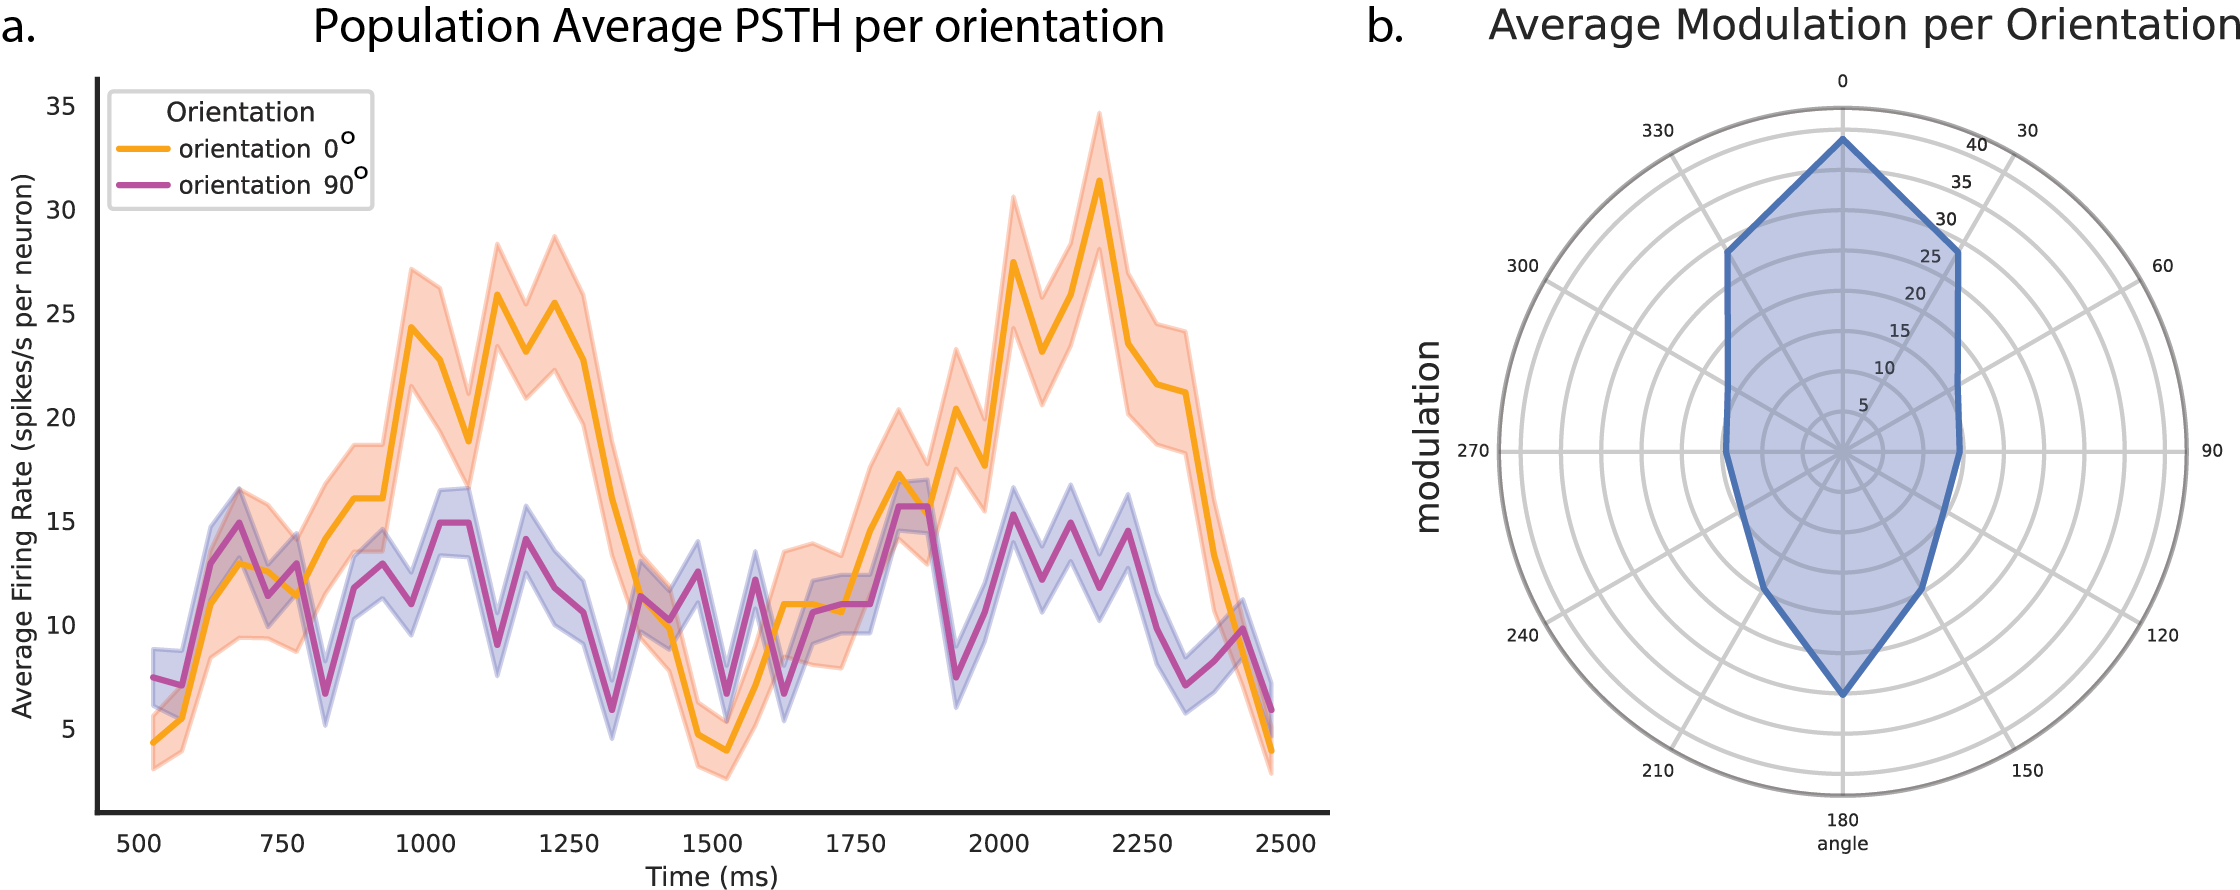
\includegraphics[width=1.0 \textwidth]{figures/figure_simple_orientation_tuning.png}
    \caption{Orientation tuning example of population ON/OFF cells at 0 and 90 degrees. The idea is to make a raster plot of the 90 a path and average modulation plot, then the same for the 0 degrees. So we have raster, under that psth  for both the 0 and the 90 degrees, and next to that a large orientation polar plot for all orientations}
    \label{fig:simple cell orientation tuning}
\end{figure}

\subsection{Polarity Invariance of Complex Cells.}
Subsequently, complex cells are created by strategically connecting these simple cells. The process began by connecting LGN cells to V1 simple cells using elliptical receptive fields and then by combining simple cells to form complex cells; we ensured phase invariance and enhanced orientation selectivity.

% Connections from LGN cells to V1 simple cells were established using a selective connection rule implemented through a connection function. This function determined whether an LGN cell's position fell within the bounds of the ON or OFF ellipse of a given V1 cell. For each LGN cell, the function checked if the cell's position was within the elliptical boundary using a mathematical condition defining point inclusion inside an ellipse based on the ellipse's centre, axes, and orientation. Once identified within the receptive field of a V1 cell, synaptic connections were established with specific weights and delays. These synaptic parameters were tuned to reflect the physiological properties of synaptic transmission observed in biological systems, with synaptic weights determining the strength of the input and delays accounting for the signal travel time between the cells.

To create a phase invariant complex cells a small number of retinotopically aligned simple cells were connected to achieve overlapping ON/OFF and OFF/ON receptive fields. The converging simple cells all had the same preferred orientation but different spatial phases creating a single complex cell. The selective connection rule played a crucial role in this process. The rule iterated over all possible simple cell sources for each target complex cell, checking for alignment in orientation and differences in phase. Synaptic connections were established between the simple cells and the complex cell, ensuring that the complex cell received inputs from a diverse set of simple cells. This convergence allowed the complex cell to respond to a range of spatial phases of a given orientation, thereby achieving phase invariance.

In the code implementation, complex cells were created by defining their receptive fields and connecting them to simple cells using a similar selective connection rule. The positions of complex cells were generated within a specified spatial grid, and their receptive fields were aligned with the preferred orientations of the contributing simple cells. The connection rule ensured that each complex cell received input from multiple simple cells with the same orientation preference but different phase preferences. This was accomplished by iterating over all potential simple cell sources for each target complex cell, establishing connections based on the orientation and phase alignment.

Through this method, elliptical receptive fields with distinct ON and OFF regions enabled V1 simple cells to become orientation-selective. By combining these simple cells to form complex cells, we achieved phase invariance, allowing complex cells to respond robustly to a given orientation regardless of the spatial phase of the input. The careful design of the spatial arrangement of the ellipses, the selective connection rules, and the convergence of simple cells onto complex cells ensured that the V1 network exhibited properties similar to those observed in biological visual systems. This approach provided a robust model for studying the mechanisms of orientation selectivity, phase invariance, and the role of specific LGN and simple cell inputs in shaping the response properties of V1 neurons.


\begin{figure}[H]
    \centering
    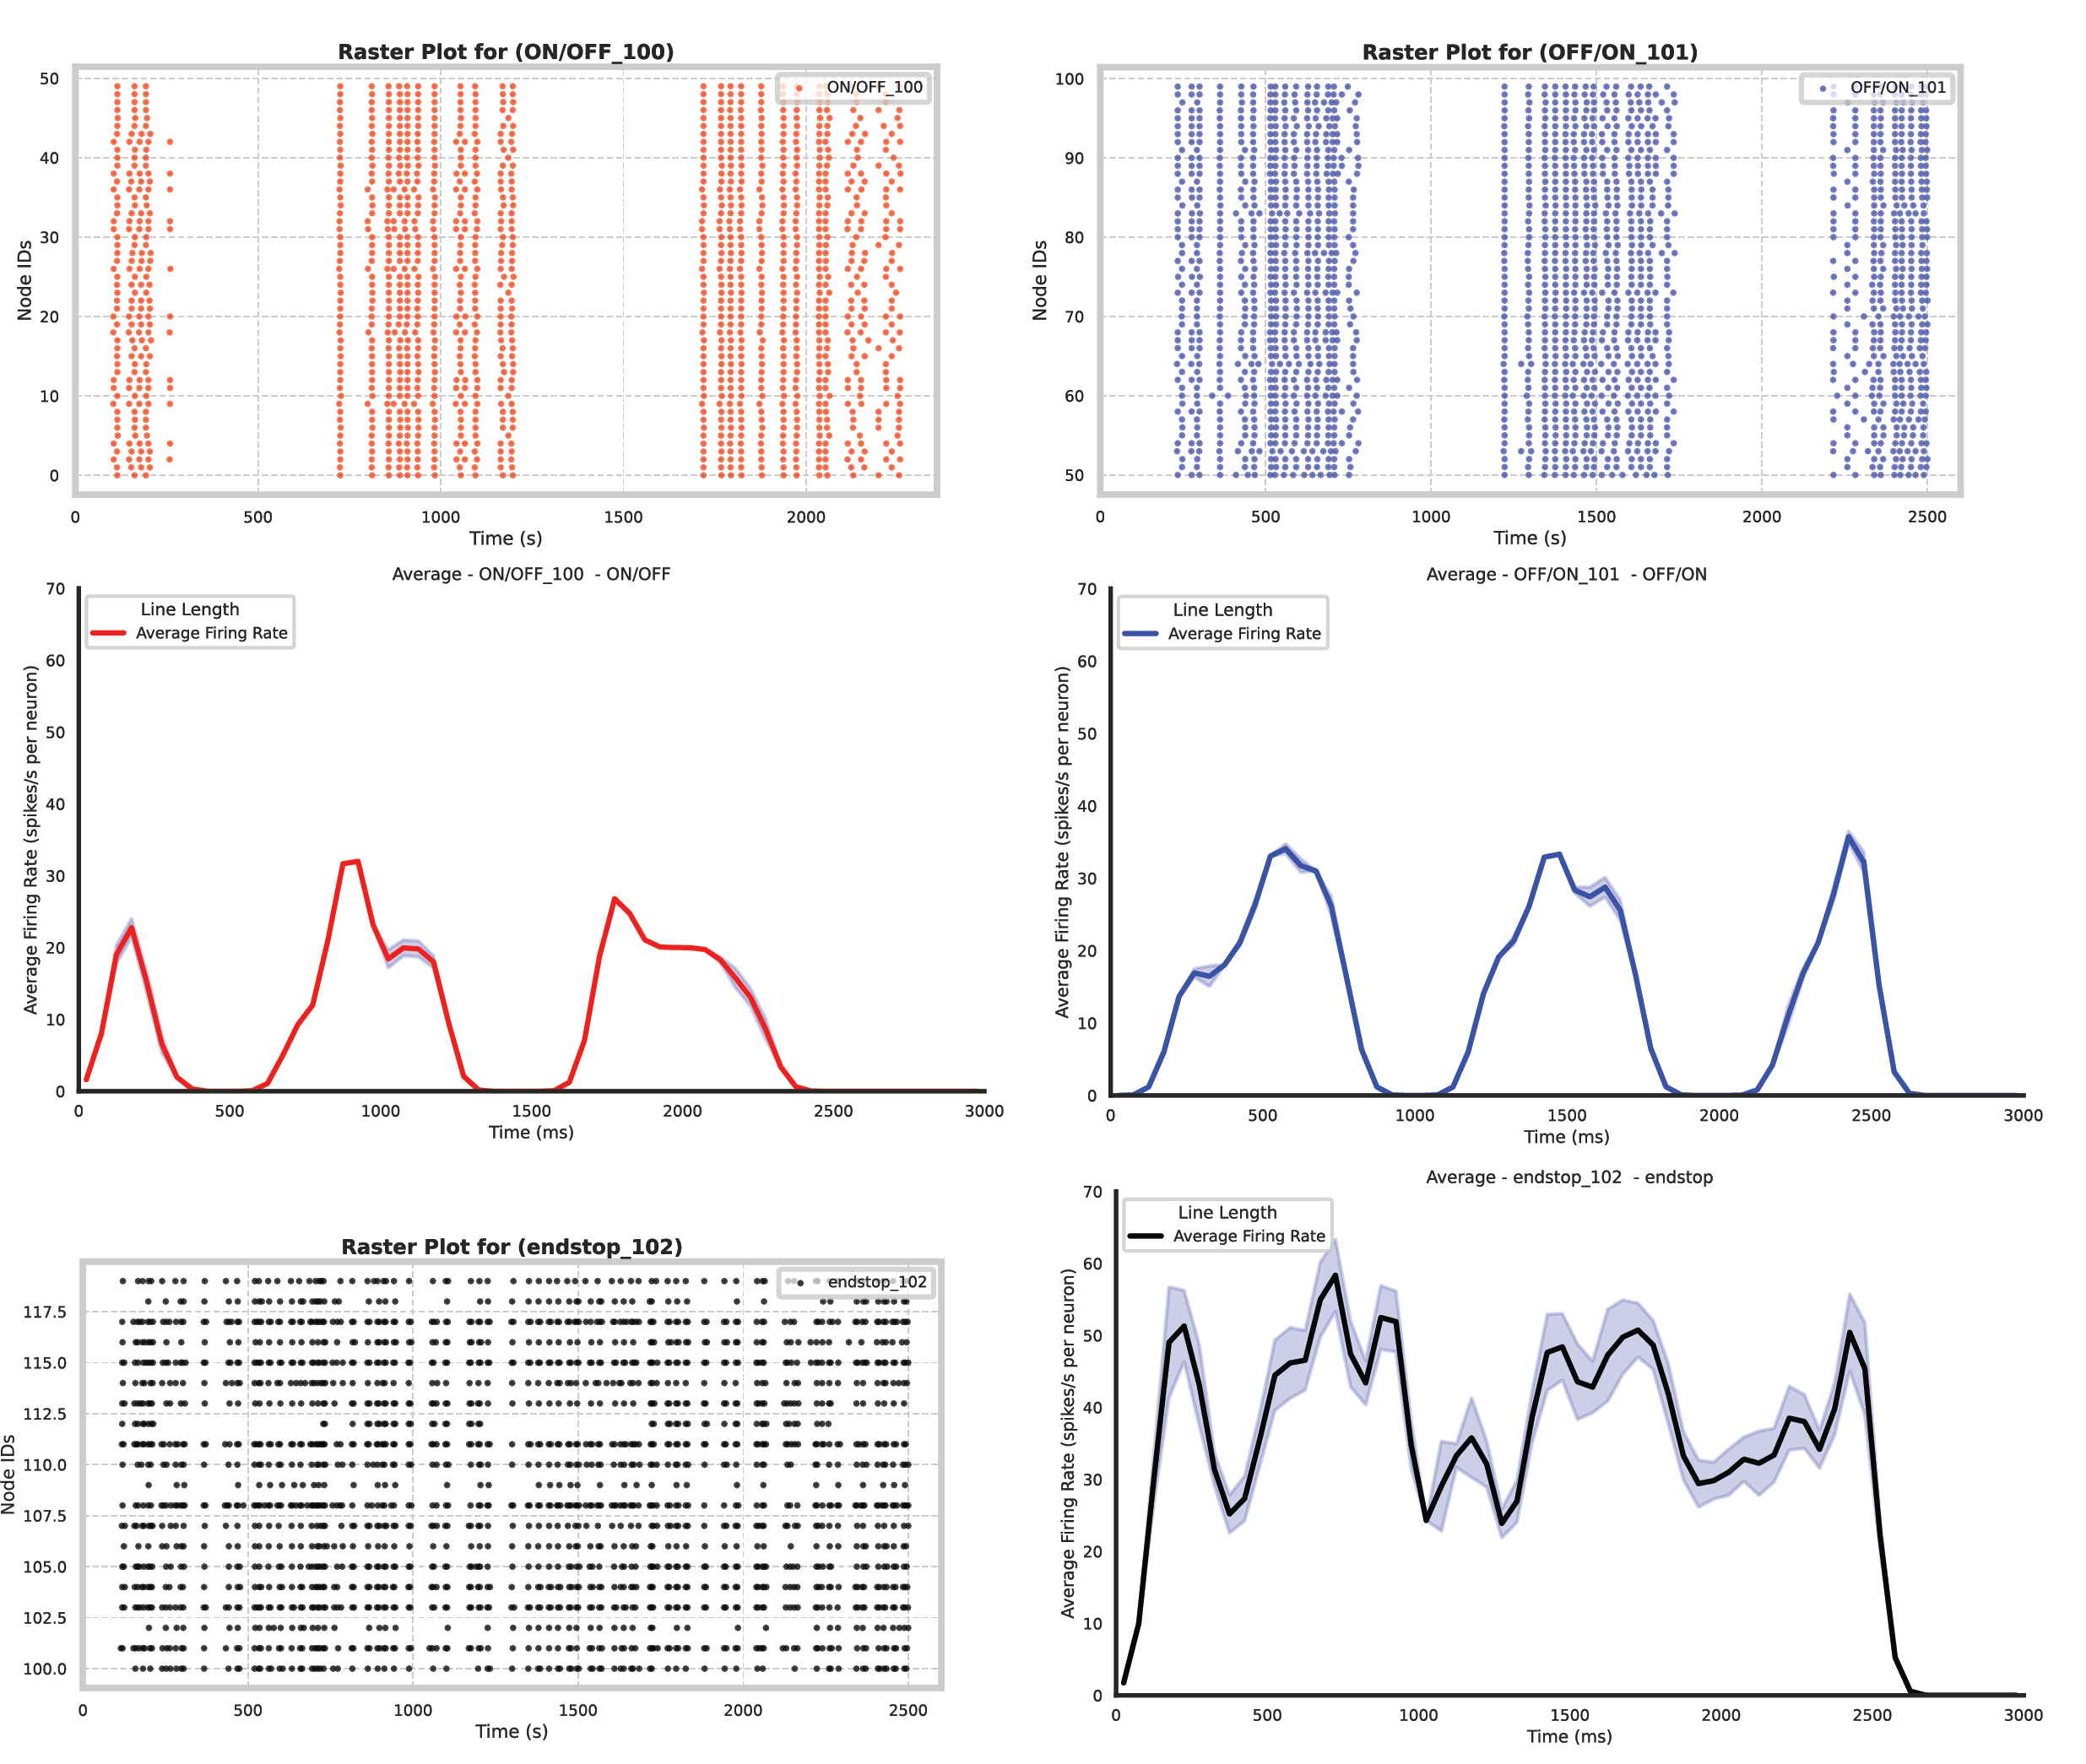
\includegraphics[width=1 \textwidth]{figures/Complex_invariancy.png}
    \caption{Polarity invariance of complex cells, 0 and 90; while maintaining the right orientation selectivity}
    \label{fig:polarity invariance}
\end{figure}

\subsection{Recurrent feedback underlying endstopping.}
In addition to creating orientation-selective and phase-invariant complex cells, I employed recurrent feedback to inhibitory cells to model the phenomenon of endstopping, a critical feature in the visual processing system. The process began with the projection of simple cells into complex cells. Specifically, simple cells with orientation-selective receptive fields were connected to complex cells that integrated inputs across different spatial phases, thus achieving phase invariance.

The next step involved the lateral displacement of these complex cells. These laterally displaced complex cells then projected to inhibitory interneurons. This displacement was crucial as it introduced a spatial offset between the excitation source and the location where inhibition would be applied, mimicking the spatial dynamics observed in cortical circuits. The inhibitory interneurons targeted by these projections played a key role in modulating the activity of the simple cells.

Once activated by the complex cells, the inhibitory cells provide feedback to the simple cells positioned directly beneath the original complex cells. This feedback loop was designed to suppress the activity of the simple cells when a stimulus extended beyond their receptive field. In more detail, as a line or bar stimulus moved across the receptive field of a simple cell and extended beyond it, the laterally displaced complex cell would activate the inhibitory interneurons. These interneurons, in turn, would inhibit the simple cells, thereby reducing their firing rate. This rapid inhibition is a hallmark of endstopping, where the neuron's response is curtailed when a stimulus exceeds the optimal length within its receptive field.

The introduction of this recurrent feedback mechanism was essential for creating endstop cells, which are specialized for detecting the endpoints of lines and bars. Endstop cells are known for their ability to signal the presence of corners, line ends, and other salient features in the visual field, making them critical for complex shape and motion perception. By implementing this feedback loop, the model could replicate the rapid decline in firing rate that characterises endstopping, providing a more accurate and nuanced representation of visual processing as seen in the primary visual cortex.

This approach highlights the importance of inhibitory feedback in fine-tuning the responses of neurons to visual stimuli, ensuring that the network could adapt to varying stimulus lengths and shapes. The recurrent feedback to inhibitory cells not only enhanced the functional properties of the model but also added a layer of biological realism by incorporating mechanisms observed in actual neural circuits. Through this detailed modelling, the network was able to exhibit advanced visual processing capabilities, closely mirroring the behaviour of endstop cells found in the visual cortex.

\begin{table}[h]
  \centering
  \caption{Connection Weights in the LIF endstop Circuit}
  %\label{tab:weights}
  \begin{tabular}{@{}llc@{}}
      \toprule
      \textbf{From} & \textbf{To} & \textbf{Weight} \\ \midrule
      Excitatory (e) & Excitatory (e) & 5.0 \\
      Excitatory (e) & Inhibitory (i) & 1.0 \\
      Inhibitory (i) & Excitatory (e) & -15.0 \\ \bottomrule
  \end{tabular}
\end{table}

\subsection{Population activity and illusory contour representation.}
In order to investigate the generation of illusory contour in the visual cortex, we used population activity models to abstract the endstopping responses of V1 neurons to visual stimuli as presented in our LIF model in a more tractable form. The population models allowed us to recreate the interlaminar endstopping microcircuits by treating each cell type as a specific population and study how multiple endstopping microcircuits collectively encoded the presence of illusory contours in a specific retinotopic coordinate of the visual field. This way we still captured the dynamic interactions between simple, complex, endstopping, and inhibitory interneurons, while providing a network of which the activity could be further integrated in a higher visual cortical area such as lateromedial cortex (LM), the second visual area in the mouse. In turn, this allowed us to examine how higher level visual feedback could provide information for V1 to induce an illusory filling in mechanism between retinotopic coordinates. Thus, abstracting the LIF model into a population model allowed for a more comprehensive view of how V1 processes visual information in the case of possible occlusion and how a illusory response can be generated to particular stimulus configurations.

\subsubsection{Overview of the population model.}
This text should describe the connectivity patterns used to shape the population model, the parameters used to define the neural dynamics, and the overall structure of the model. It should also explain how the model was used to simulate the generation of illusory contours in the visual cortex and how the results were interpreted to gain insights into the neural mechanisms underlying this phenomenon.
\begin{figure}[H]
  \centering
  % \includegraphics[width=1 \textwidth]{figures/Population_model.png}
  \caption{Population model of V1, integrating a microcircuit of simple, complex, endstopping and inhibitory cells into LM pattern cells that give feedback to V1 for filling in an illusory contour response.}
  \label{fig:population model}
\end{figure}


\subsubsection{PyRates Library and population parameters.}
In our study, we employed a Wilson and Cowan neural mass model using the PyRates library to simulate neural dynamics. This model helps us understand how groups of neurons interact with each other over time. It consists of several key components and parameters that we will explain in detail.

First, we define an operator called the synaptic excitation operator (\texttt{se\_op}). This operator uses a sigmoid function to model the process of synaptic excitation, which is how neurons get excited and send signals. The equation for this operator is:
\[
m = \operatorname{sigmoid}(s \cdot (r_{\mathrm{in}} + r_{\mathrm{ext}} - \theta)) - \operatorname{sigmoid}(-s \cdot \theta),
\]
where \( m \) represents the output signal from the neuron. The term \(\operatorname{sigmoid}\) is a mathematical function that smoothly limits the output between 0 and 1, mimicking the neuron's firing rate. The parameter \( s \) controls the steepness of the sigmoid curve and is set to 1.0, meaning it defines how quickly the neuron responds to input. The parameter \(\theta\) is a threshold set to 2.0, which the input must exceed for the neuron to start firing significantly. The inputs \( r_{\mathrm{in}} \) and \( r_{\mathrm{ext}} \) represent signals coming from other neurons and external sources, respectively, and both are initially set to 0.0.

We also have a variation called the synaptic inhibition operator (\texttt{si\_op}). This operator works similarly but models inhibitory signals, which reduce neuron activity. Its equation is similar, but with different parameters: \( s \) is set to 2.0, making the response steeper, and \( \theta \) is set to 2.5, meaning a higher threshold for inhibition.

Next, we describe the rate operator (\texttt{rate\_op}). This operator models the rate of change in neural activity over time using the differential equation:
\[
r' = \frac{-r + (1.0 - k \cdot r) \cdot m}{\tau}.
\]
Here, \( r \) is the current activity level of the neuron, initially set to 0.0. The parameter \( k \) is set to 1.0 and influences how the neuron's activity decreases over time. The term \( \tau \) represents the time constant set to 10.0, which defines how quickly the neuron activity responds to changes. The input \( m \) is the signal calculated by the excitation or inhibition operators.

To model neural populations, we use node templates. The excitatory population node template (\texttt{exc\_pop}) combines the rate operator and the synaptic excitation operator to represent a group of excitatory neurons, which promote activity in the network. Conversely, the inhibitory population node template (\texttt{inh\_pop}) combines the rate operator and the synaptic inhibition operator to represent a group of inhibitory neurons, which suppress activity in the network.

Circuit templates define the network structure of the model. The Wilson-Cowan circuit template (\texttt{WC}) consists of two nodes: an excitatory population (\texttt{e}) and an inhibitory population (\texttt{i}). The parameters used in the model are summarized in Table~\ref{tab:parameters}.

\begin{table}[h]
    \centering
    \caption{Parameters of the Wilson-Cowan Neural Mass Model}
    \label{tab:parameters}
    \begin{tabular}{@{}lll@{}}
        \toprule
        \textbf{Parameter} & \textbf{Description} & \textbf{Value} \\ \midrule
        \( s \) & Steepness of the sigmoid curve (excitation) & 1.0 \\
        \( \theta \) & Threshold for excitation & 2.0 \\
        \( r_{\mathrm{in}} \) & Input from other neurons & 0.0 \\
        \( r_{\mathrm{ext}} \) & External input & 0.0 \\
        \( s \) (inhibition) & Steepness of the sigmoid curve (inhibition) & 2.0 \\
        \( \theta \) (inhibition) & Threshold for inhibition & 2.5 \\
        \( r \) & Current activity level & 0.0 \\
        \( k \) & Decay parameter for activity & 1.0 \\
        \( \tau \) & Time constant & 10.0 \\ \bottomrule
    \end{tabular}
\end{table}

The connections (edges) between these nodes are specified with weights that determine the strength and type of influence they exert on each other. The weights for these connections are as follows: the rate output \( r \) of the excitatory node feeds back into its own synaptic excitation input \( r_{\mathrm{in}} \) with a weight of 15.0, the rate output \( r \) of the excitatory node feeds into the synaptic inhibition input \( r_{\mathrm{in}} \) of the inhibitory node with a weight of 15.0, the rate output \( r \) of the inhibitory node reduces activity in the excitatory node by feeding into its synaptic excitation input \( r_{\mathrm{in}} \) with a weight of -15.0, and the rate output \( r \) of the inhibitory node also self-regulates by feeding back into its own synaptic inhibition input \( r_{\mathrm{in}} \) with a weight of -4.0.

These detailed specifications allow us to simulate complex neural dynamics, capturing both excitatory and inhibitory interactions within the network. By adjusting the weights and incorporating these parameters, we can flexibly and realistically represent neural behavior and understand how neurons interact and influence each other over time.


Circuit templates define the network structure of the model. The Wilson-Cowan circuit template (\texttt{WC}) consists of two nodes: an excitatory population (\texttt{e}) and an inhibitory population (\texttt{i}). The connections (edges) between these nodes are specified with weights that determine the strength and type of influence they exert on each other. These weights are outlined in Table~\ref{tab:weights}.

\begin{table}[h]
    \centering
    \caption{Connection Weights in the Wilson-Cowan Circuit}
    \label{tab:weights}
    \begin{tabular}{@{}llc@{}}
        \toprule
        \textbf{From} & \textbf{To} & \textbf{Weight} \\ \midrule
        Excitatory (e) & Excitatory (e) & 15.0 \\
        Excitatory (e) & Inhibitory (i) & 15.0 \\
        Inhibitory (i) & Excitatory (e) & -15.0 \\
        Inhibitory (i) & Inhibitory (i) & -4.0 \\ \bottomrule
    \end{tabular}
\end{table}

These detailed specifications allow us to simulate complex neural dynamics, capturing both excitatory and inhibitory interactions within the network. By adjusting the weights and incorporating synaptic plasticity models, we can flexibly and realistically represent neural behavior and understand how neurons interact and influence each other over time.

\section{Results}
\subsection{LIF Endstopped Receptive Field properties.}
%Research Question: Role of recurrent inhibition in creating balanced activity during stimulus presentation. 
To examine the role of recurrent inhibition in the process of endstopping we constructed a neural model consisting of a microcircuit of simple cells, complex cells and inhibitory interneurons. A simple cell population of a particular retinotopic coordinate is connected to a complex cell which creates an inhibitory feedback loop by connecting to an inhibitory population that inhibits the activity of a neighbouring simple cell population. This configuration allows us to simulate the behaviour of endstopped complex cells in response to different line segments of varying lengths and orientations. The results in Figure~\ref{fig:complex_cell_responses} confirmed that the endstop cell was spiking maximally when a line bar is positioned within its receptive field. However, this activity is then inhibited when the line extends into the receptive field of an adjacent complex cell. This decrease in firing rate was attributed to the inhibition from the recurrent inhibitory population. 


\begin{figure}[h]
    \centering
    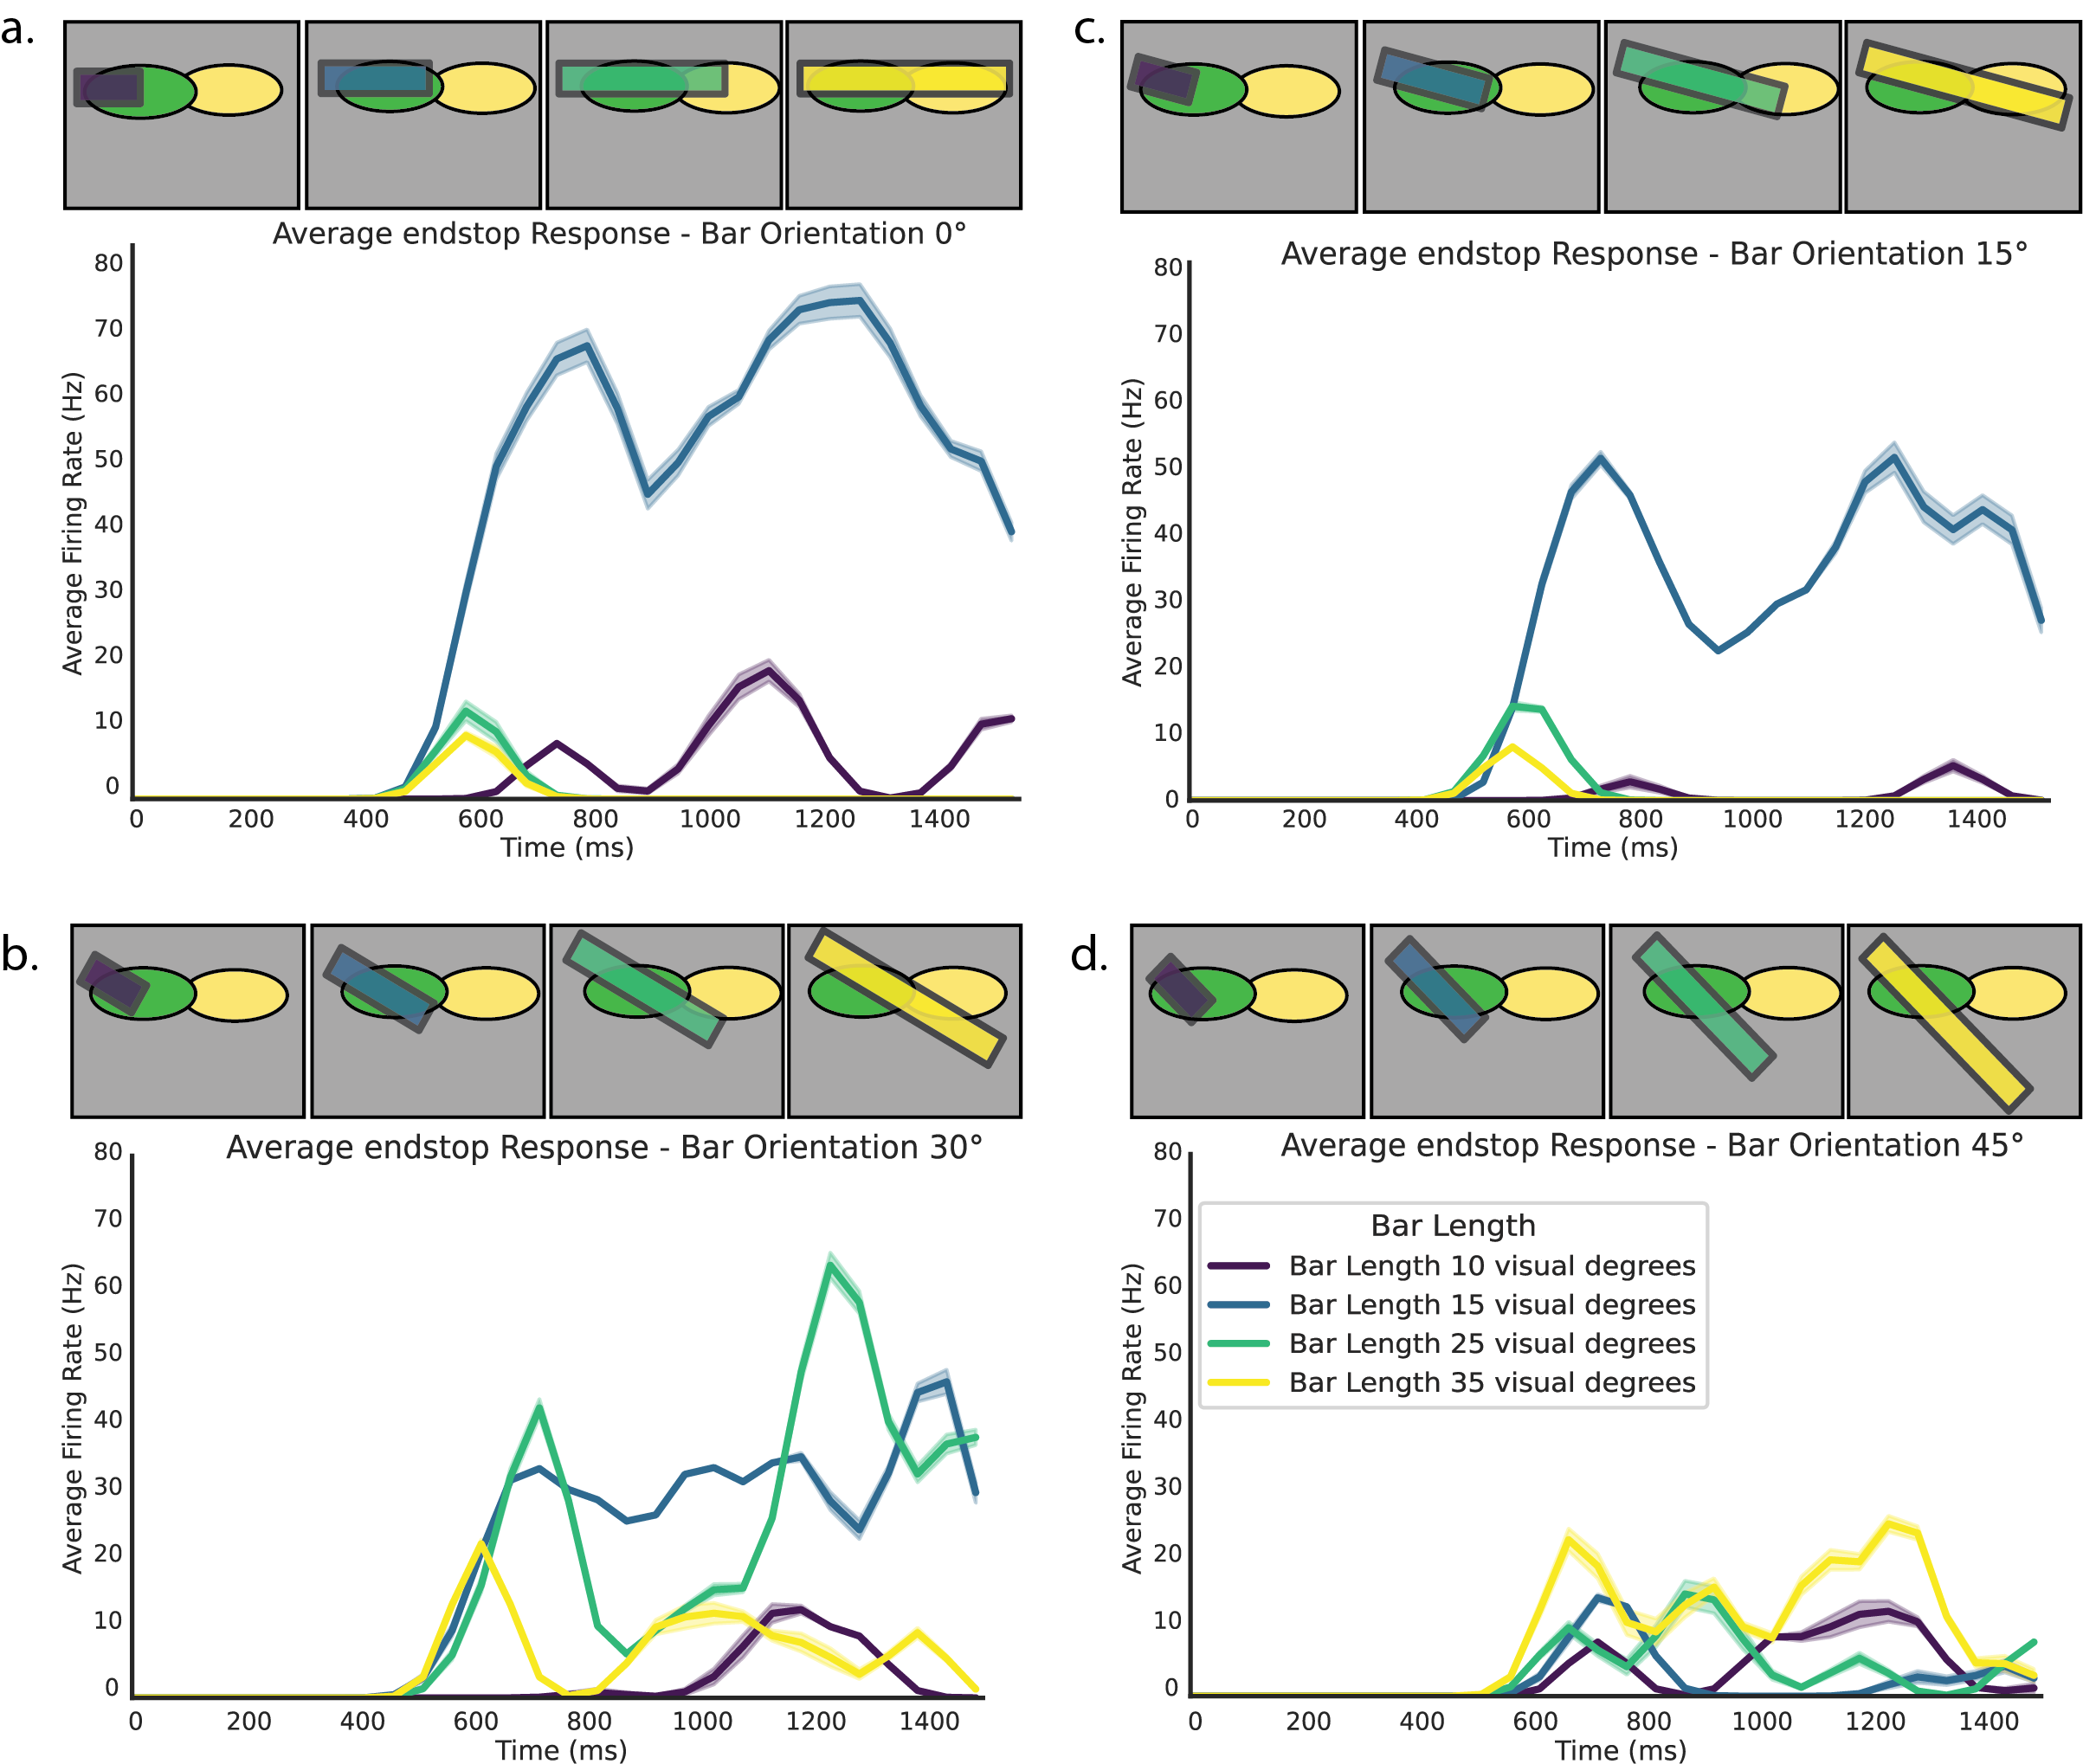
\includegraphics[width=1 \textwidth]{./figures/LIF_endstopping_length_orientation.png}
    \caption{Responses of the endstopped complex cells to different line segment lengths. The x-axis represents the length of the line segment, and the y-axis represents the firing rate of the complex cell.}
    \label{fig:endstopping}
\end{figure}


We presented the model with various line segments of different lengths and orientations to observe the behavior of the endstopped complex cells. The results showed that the complex cell spiked maximally when a line bar was within its receptive field. As the length of the line segment increased and extended into the receptive field of the neighboring complex cell, the firing rate of the endstopped complex cell decreased. This decrease in firing rate was attributed to the inhibition from the recurrent inhibitory population.

Figure~\ref{fig:complex_cell_responses} illustrates the firing rates of the endstopped complex cells in response to line segments of varying lengths. The x-axis represents the length of the line segment, and the y-axis represents the firing rate of the complex cell. The results demonstrated that without recurrent inhibition, the complex cell continued to spike even when the line segment extended into the receptive field of the neighboring complex cell. Conversely, with recurrent inhibition, the activity of the complex cell was suppressed when the line segment extended beyond its optimal length.

The recurrent inhibition consistently resulted in a decrease in the firing rate of the endstopped complex cell when the stimulus extended into the receptive field of the adjacent complex cell. The data consistently showed that recurrent inhibition played a crucial role in balancing neural activity during stimulus presentation.


  \begin{figure}[h]
      \centering
      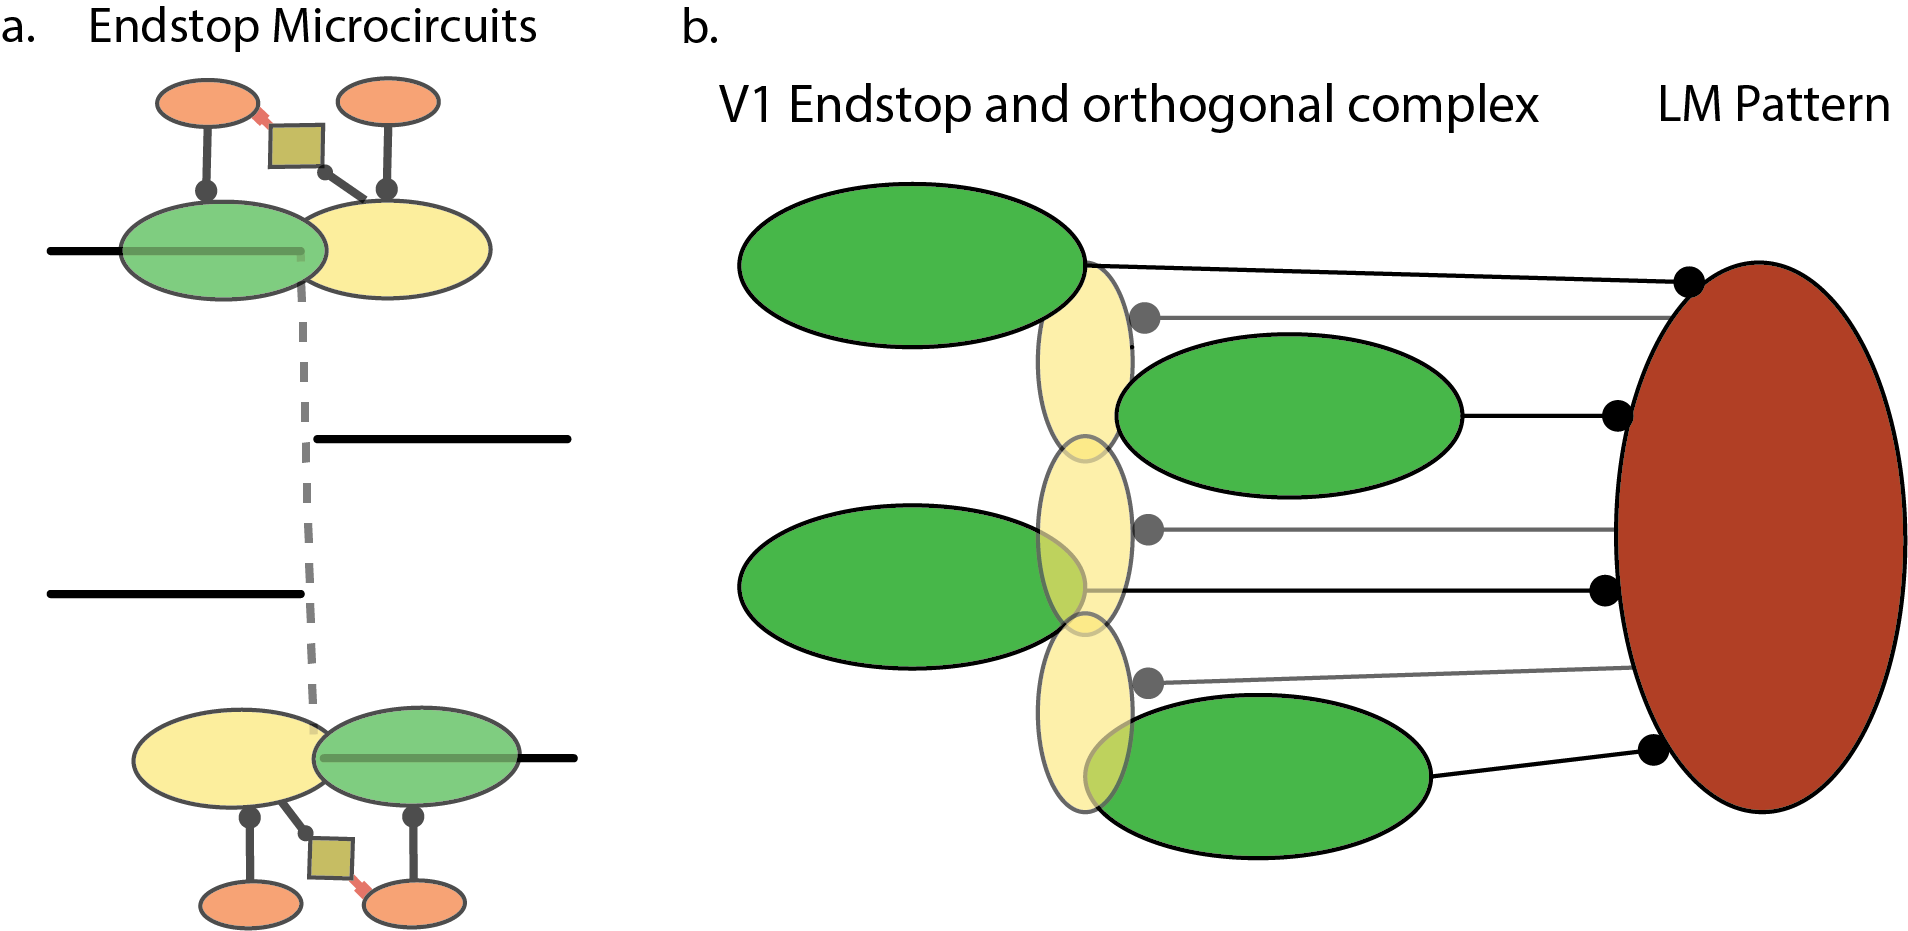
\includegraphics[width=1 \textwidth]{./figures/illusory_filling.png}
      \caption{Responses of the endstopped complex cells to different line segment lengths. The x-axis represents the length of the line segment, and the y-axis represents the firing rate of the complex cell.}
      \label{fig:complex_cell_responses}
  \end{figure}



  \subsubsection{Use average firing rate or modulation for endstopping quantification.}

\subsection{Population activity illusory contours}

\subsection{Representation real contours vs illusory contours in the model}


\newpage
\section{Discussion}

\subsection{Model predictions; results in the literature.}
  \subsubsection{Recurrent inhibitory activty balances activity needed for stable endstopping.}
  Our model demonstrates that recurrent inhibition plays a crucial role in balancing neural activity during stimulus presentation, thereby stabilizing the endstopping phenomenon. In a strictly feedforward network, such stabilization is not possible. The presence of recurrent inhibition ensures that the activity of the endstopped complex cells is modulated appropriately based on the spatial extent of the stimulus. The findings provide a clear answer to the research question by demonstrating that recurrent inhibition stabilizes the endstopping feature in the neural model, which is not achievable in a strictly feedforward network. The consistent suppression of the complex cell's activity by the recurrent inhibitory population validates the importance of recurrent inhibition in the model.

  \subsubsection{Real vs illusory contour representation}
  Electrophysiological it seems that the L4 simple cells are dominated by feedforward input and thus should not directly be influenced by illusory contours, the current model is indeed setup so that from L2/3 the endstopped cells converge onto higher visual areas and which send feedback to deeper layers of the visual cortex. 
  Electrophysiology, deeper layers more active or superficial layers? should be feedback, normally feedback from higher visual areas target deeper layers, but in the case of illusory contours, it seems that feedback from higher visual areas target superficial layers. (need to check this in the literature, done in mice: Wyatte, filling in process; Shin IC encoder where?, Pak et al. 2019, feedback from LM to V1 superficial layers)

\subsection{Feedback allows for orientation interpolation for curved surfaces.}
As seen in the results with current mass models it is possible to instruct orientation specific illusory contours, however in other electrophysiological studies it is clear that there are cases in which the illusory contour is curved. This is not possible with the current model, but it is possible to extend the model to include feedback from higher visual areas to V1 to allow for orientation interpolation. This would allow for the model to generate curved illusory contours, which would be a more accurate representation of the visual system. A possible neuronal mechanism that would result in curved illusory contour is a broad feedback response that integrates multiple orientations around the inducing orientation. In other words, the orientation selective feedforward input from the endstopped cells to the higher visual Pattern cells would be integrated and give feedback to closely matched cells instead of only the same orientation tuning as in the current model. Additionally, known feedback mechanisms to local inhibitory cells in L2/3 could also be included for a more rich feedback response that fills in between occluding visual features.
\subsection{Limitations}
\subsubsection{Deep learning optimisation}
The current model was tuned by hand to achieve the desired endstopping behaviour, combining multiple hierarchical levels of neuronal complexity. In future work, deep learning optimization techniques could be employed to automatically tune the model parameters and connectivity weights to achieve the desired endstopping behaviour. This would allow for a more systematic exploration of the parameter space and potentially uncover novel configurations that enhance the model's performance. Additionally, the use of deep learning optimization could help identify the most critical parameters and connections that contribute to endstopping, providing valuable insights into the underlying neural mechanisms. 

This would make it possible to formulate a model consisting only of LIF cells in contrast to the mass neural models used in the current model. Additionally, the use of deep learning optimisation would make it possible to simulate the model on a larger scale, but also to simulate network responses to more continuously altered input configuration, testing it's robustness better.



\newpage
\printbibliography

\end{document}